\let\negmedspace\undefined
\let\negthickspace\undefined
\documentclass[journal]{IEEEtran}
\usepackage[a5paper, margin=10mm, onecolumn]{geometry}
%\usepackage{lmodern} % Ensure lmodern is loaded for pdflatex
\usepackage{tfrupee} % Include tfrupee package

\setlength{\headheight}{1cm} % Set the height of the header box
\setlength{\headsep}{0mm}     % Set the distance between the header box and the top of the text

\usepackage{gvv-book}
\usepackage{gvv}
\usepackage{cite}
\usepackage{amsmath,amssymb,amsfonts,amsthm}
\usepackage{algorithmic}
\usepackage{graphicx}
\usepackage{textcomp}
\usepackage{xcolor}
\usepackage{txfonts}
\usepackage{listings}
\usepackage{enumitem}
\usepackage{mathtools}
\usepackage{gensymb}
\usepackage{comment}
\usepackage[breaklinks=true]{hyperref}
\usepackage{tkz-euclide} 
% \usepackage{gvv}                                        
\def\inputGnumericTable{}                                 
\usepackage[latin1]{inputenc}                                
\usepackage{color}                                            
\usepackage{array}                                            
\usepackage{longtable}                                       
\usepackage{calc}                                             
\usepackage{multirow}                                         
\usepackage{hhline}                                           
\usepackage{ifthen}                                           
\usepackage{lscape}
\begin{document}

\bibliographystyle{IEEEtran}
\vspace{3cm}

\title{10.3.5.1.4}
\author{EE24BTECH11029 - J SHRETHAN REDDY}
\maketitle
% \newpage
% \bigskip
{\let\newpage\relax\maketitle}

\renewcommand{\thefigure}{\theenumi}
\renewcommand{\thetable}{\theenumi}
\setlength{\intextsep}{10pt} % Space between text and floats


\numberwithin{equation}{enumi}
\numberwithin{figure}{enumi}
\renewcommand{\thetable}{\theenumi}
\textbf{Question}:\\
Solve the system of linear equations:
\begin{align}
    x - 3y - 7 &= 0 \\
    3x - 3y - 15 &= 0
\end{align}
\textbf{Step 1: Represent the system in matrix form} \\ 
The system of equations can be written as:  
\begin{align}  
A \mathbf{x} = \mathbf{b},  
\end{align}  
where  
\begin{align}
    A=\myvec{1 & -3 \\ 
             3 & -3} ,
    x=\myvec{x\\y} ,
    b=\myvec{7 \\ 15}
\end{align}
\textbf{Step 2: Perform LU Decomposition} \\ 
We decompose the matrix $A$ into the product of a lower triangular matrix $L$ and an upper triangular matrix $U$, i.e.,  
\begin{align}  
A = LU
\end{align}  
where  
\begin{align}  
L=\myvec{1 & 0\\l_{21} & 1},
U=\myvec{u_{11} & u_{12}\\0 & u_{22}}
\end{align}

Now, let's compute the LU decomposition step by step.  

First, we find the elements of $U$ and $L$:  
\begin{align}  
u_{11} = a_{11} = 1, u_{12} = a_{12} = -3.  
\end{align}  
Next, we compute $l_{21}$ and $u_{22}$:  
\begin{align}  
l_{21} = \frac{a_{21}}{u_{11}} = \frac{3}{1} = 3,  
\end{align}  
\begin{align}  
u_{22} = a_{22} - l_{21} u_{12} = -3 - \brak{3} \times \brak{-3} = 6.  
\end{align}  
So the LU decomposition is:  
\begin{align}
    L=\myvec{1 & 0\\1 & 1},
    U=\myvec{1 & -3\\0 & 2},
\end{align}
\textbf{Step 3: Solve for $\mathbf{x}$ using $LU$ decomposition}  \\
Now we solve the system in two steps using forward substitution and backward substitution.  

First, solve $L \mathbf{y} = \mathbf{b}$ for $\mathbf{y}$:  
\begin{align}  
     L=\myvec{1 & 0\\3 & 1}\myvec{y_1\\y_2} = \myvec{7\\15}
\end{align}  
This gives:  
\begin{align}  
y_1 = 7, 3y_1 + y_2 = 15 \\
 y_2 = -6.  
\end{align}  
Thus, $\mathbf{y} = \begin{pmatrix} 7 \\ -6 \end{pmatrix}$.  

Next, solve $U \mathbf{x} = \mathbf{y}$ for $\mathbf{x}$:  
\begin{align}
    U=\myvec{1 & -3\\0 & 6}\myvec{x \\ y} = \myvec{7\\-6}
\end{align}
This gives:  
\begin{align}  
6y = -6 \Rightarrow y = -1, \\  
x - 3y = 7\Rightarrow x= 4.  
\end{align}  

Thus, the solution is $x = 4$ and $y = -1$.  

\textbf{LU Decomposition using Doolittle's algorithm}:  \\
The LU decomposition can be efficiently computed using Doolittle's algorithm. This method generates the matrices $L$ (lower triangular) and $U$ (upper triangular) such that $A = LU$. The elements of these matrices are calculated as follows: \\  
Elements of the $U$ Matrix: \\  
For each column $j$:  
\begin{align}  
U_{ij} = A_{ij} \text{ if } i = 0, \\  
U_{ij} = A_{ij} - \sum_{k=0}^{i-1} L_{ik} U_{kj} \text{ if } i > 0.  
\end{align}  
Elements of the $L$ Matrix: \\  
For each row $i$:  
\begin{align}  
L_{ij} = \frac{A_{ij}}{U_{jj}} \text{ if } j = 0, \\  
L_{ij} = \frac{A_{ij} - \sum_{k=0}^{j-1} L_{ik} U_{kj}}{U_{jj}} \text{ if } j > 0.  
\end{align}  

This systematic approach ensures that the matrix $A$ is decomposed into $L$ and $U$ without requiring row swaps, provided $A$ is nonsingular.  
\begin{figure}[h!]
   \centering
   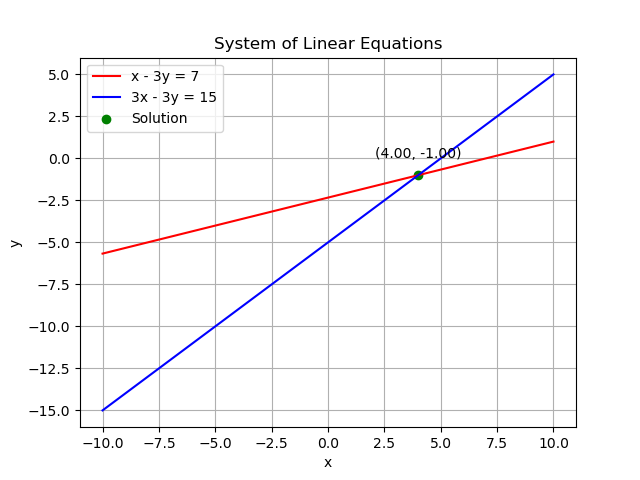
\includegraphics[width=1\columnwidth]{figure/fig.png}
   \caption{Solving the system of equations}
   \label{stemplot}
\end{figure}


\end{document}

